\documentclass{beamer}

\usepackage{listings}
\usepackage{xcolor}
\usepackage{multicol}
\usepackage{amsmath}

\definecolor{codegreen}{rgb}{0,0.6,0}
\definecolor{codegray}{rgb}{0.5,0.5,0.5}
\definecolor{codepurple}{rgb}{0.58,0,0.82}
\definecolor{backcolour}{rgb}{0.95,0.95,0.92}

\lstdefinestyle{mystyle}{
    %backgroundcolor=\color{backcolour}, 
    commentstyle=\color{codegreen},
    keywordstyle=\color{magenta},
    numberstyle=\tiny\color{codegray},
    stringstyle=\color{codepurple},
    basicstyle=\ttfamily\footnotesize,
    breakatwhitespace=false,         
    breaklines=true,                 
    captionpos=b,                    
    keepspaces=true,                 
    numbers=left,                    
    numbersep=5pt,                  
    showspaces=false,                
    showstringspaces=false,
    showtabs=false,                  
    tabsize=2
}

\lstset{style=mystyle}

\usepackage{hyperref}
\hypersetup{
    colorlinks=true,
    linkcolor=blue,
    filecolor=magenta,      
    urlcolor=cyan
}

\urlstyle{same}

\title{2: Data Structures and Libraries}
\author{CPCFI}
\institute{UNAM's School of Engineering}
\date{2021 \\ \vspace{0.5cm} \scriptsize{Based on: Halim S., Halim F.\textit{Competitive Programming 3}}. Handbook for ACM ICPC and IOI Contestants. 2013}

\begin{document}

\frame{\titlepage}

\AtBeginSection[]
{
  \begin{frame}
    \frametitle{Table of Contents}
    \tableofcontents[currentsection]
  \end{frame}
}

%-------------------------------------------------------------------------------------------
%-------------------------------------------------------------------------------------------
%-------------------------------------------------------------------------------------------
\section{2.3  Non-Linear Data Structures with Built-in Libraries}

%-------------------------------------------------------------------------------------------
%-------------------------------------------BST---------------------------------------------
%-------------------------------------------------------------------------------------------
\subsection{Balanced Binary Search Tree (BST)}
\begin{frame}{Balanced Binary Search Tree - BST}
    \begin{figure}
        \centering
        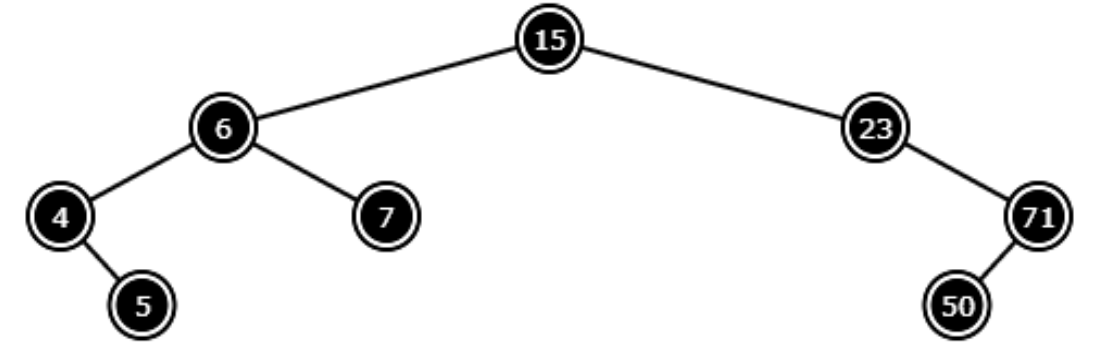
\includegraphics[scale=0.4]{imgs/2.3/bst/bst.png}
    \end{figure}
\end{frame}

\begin{frame}[fragile]{Balanced Binary Search Tree}
    \begin{itemize}
    	\item A Binary Search Tree (BST) is a tree where each vertex has at most two children nodes that satisfy the BST Property
		    \begin{figure}
		        \centering
    		    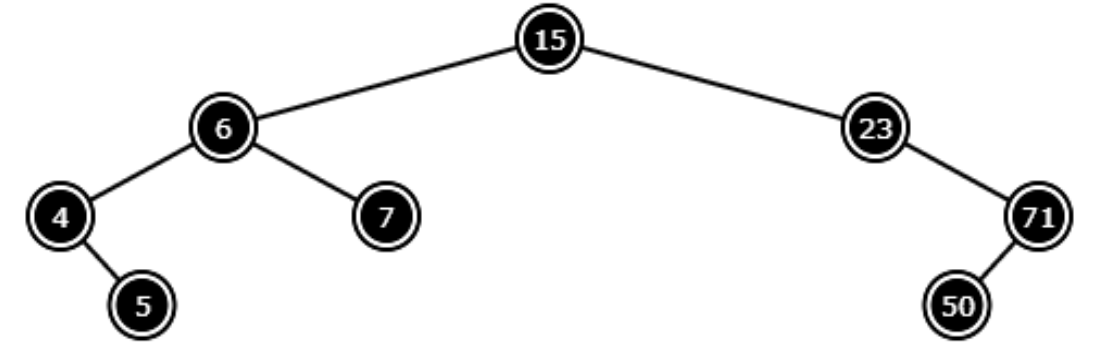
\includegraphics[scale=0.25]{imgs/2.3/bst/bst.png}
	    	\end{figure}
        \item \textbf{BST Property}: Tree with a root at $x$ where each value $v$:
            \begin{itemize}
                \item On the left of $x$ holds that $ v < x$
                \item On the right of $x$ holds that $ v \geq x$
            \end{itemize}
         \item \verb|C++ STL map|: stores \textit{key} $\rightarrow$ \textit{value}
         \item \verb|C++ STL set|: only stores \textit{key}
         \item \color{red} \verb|ch2_05_map_set.cpp| \color{black}
    \end{itemize}
\end{frame}

\begin{frame}[fragile]
\frametitle{BST as Table ADT}
	\begin{itemize}
         \item A BST is an efficient and dynamic\footnote{Data structure that keeps efficiency even in the presence of many update operations} data structure to implement a Table or Map ADT
         \item Table ADT must support:
         	\begin{itemize}
				\item \verb|search(v)|
				\item \verb|insert(v)|
				\item \verb|remove(v)|
				\item \verb|min()|, \verb|max|
				\item \verb|successor(v)|, \verb|predecessor(v)|
			\end{itemize}
		\item These operations run in $O(n\log n)$
	\end{itemize}
\end{frame}

\begin{frame}[fragile]
\frametitle{BST - Vertex Attributes}
	\begin{figure}
		\centering
		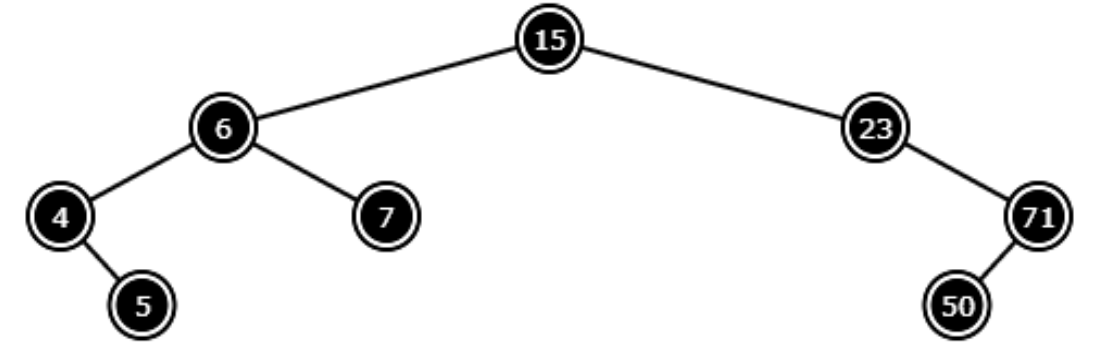
\includegraphics[scale=0.4]{imgs/2.3/bst/bst.png}
	\end{figure}
	\begin{itemize}
		\item Each vertex has at least 4 attributes:
			\begin{enumerate}
				\item \verb|parent|
				\item \verb|left|
				\item \verb|right|
				\item \verb|key|, \verb|value|, \verb|data|
			\end{enumerate}
	\end{itemize}
\end{frame}

\begin{frame}[fragile]
\frametitle{BST - Operations}
	\begin{enumerate}
		\item Query operations
			\begin{itemize}
				\item \verb|Search(v)|
				\item \verb|Predecessor(v)|, \verb|Successor(v)|
				\item Inorder traversal
			\end{itemize}
		\item Update operations
			\begin{itemize}
				\item \verb|Insert(v)|
				\item \verb|Remove(v)|
				\item Create BST
			\end{itemize}
	\end{enumerate}
\end{frame}

\begin{frame}[fragile]
\frametitle{BST - Query Operations I}
	\begin{itemize}
	\item \verb|search(v)|: \color{blue} $O(h)$ \color{black} \footnote{$h$ is the height of the tree}
		\begin{itemize}
			\item Set the current vertex to the root. Then, check if the current vertex is smaller, equal or larger than \verb|v|, depending on the answer, update the current vertex to the left or right child of the root
			\item Similarly, we can find the \textbf{minimum} or the \textbf{maximum} of a BST by going all the way to the left or right of the BST
		\end{itemize}
	\end{itemize}
\end{frame}

\begin{frame}[fragile]
\frametitle{BST - Query operations II}
	\begin{itemize}
		\item \verb|predecessor(v)|: \color{blue} $O(h)$ \color{black}
			\begin{itemize}
				\item If \verb|v| has a left subtree, then the predecessor is the maximum element of the left subtree
				\item If \verb|v| does not have a left subtree, then we need to iterate over its ancestors (parents) to find the first vertex \verb|w| that is smaller than \verb|v|
				\item If \verb|v| is the minimum of the BST, \verb|v| does not have a predecessor
			\end{itemize}
		\item \verb|successor(v)|: \color{blue} $O(h)$ \color{black}
			\begin{itemize}
				\item If \verb|v| has a right subtree, then the successor is minimum element of the right subtree
				\item If \verb|v| does not have a right subtree, then we need to look for the first vertex \verb|w| that is greater than \verb|v|
				\item If \verb|v| is the maximum of the BST, \verb|v| does not have a successor
			\end{itemize}
	\end{itemize}
\end{frame}

\begin{frame}[fragile]
\frametitle{BST - Query operations III}
	\begin{itemize}
		\item Inorder traversal
			\begin{itemize}
				\item Visit order:
					\begin{enumerate}
						\item Left subtree
						\item Root
						\item Right subtree
					\end{enumerate}
				\item Obtains the list of sorted integers inside the BST
				\item \color{blue} $O(n)$ \color{black}
			\end{itemize}
		\item Preorder traversal	
			\begin{itemize}
				\item Visit order:
					\begin{enumerate}
						\item Root
						\item Left subtree
						\item Right subtree
					\end{enumerate}
			\end{itemize}
		\item Postorder traversal
			\begin{itemize}
				\item Visit order:
					\begin{enumerate}
						\item Left subtree
						\item Right subtree
						\item Root
					\end{enumerate}
			\end{itemize}
	\end{itemize}
\end{frame}

\begin{frame}[fragile]
\frametitle{BST - Update operations I}
	\begin{itemize}
		\item \verb|insert(v)|: \color{blue} $O(h)$ \color{black}
			\begin{itemize}
				\item Follow a similar approach to \verb|search(v)| but instead of reporting that the vertex does not exist, create a new vertex in the insertion point
			\end{itemize}
	\end{itemize}
\end{frame}

\begin{frame}[fragile]
\frametitle{BST - Update operations II}
	\begin{itemize}
		\item \verb|remove(v)|: \color{blue} $O(h) \;+ $ \color{black}, three possible cases:
			\begin{enumerate}
				\item Vertex \verb|v| is a leaf vertex: \color{red} $O(1)$ \color{black}
						\begin{itemize}
							\item Simply remove the vertex (parent's left or right child should point to \verb|null|)
						\end{itemize}
				\item Vertex \verb|v| is an internal or root vertex with one child: \color{red} $O(1)$ \color{black}
					\begin{itemize}
						\item Connect \verb|v|'s only child with \verb|v|'s parent
					\end{itemize}
				\item Vertex \verb|v| is an internal or root vertex with two children: \color{red} $O(h)$ \color{black}
					\begin{itemize}
						\item Replace \verb|v| with its successor
						\item Delete its duplicated successor in its right subtree
					\end{itemize}
			\end{enumerate}
	\end{itemize}
\end{frame}


%-------------------------------------------------------------------------------------------
%-------------------------------------------Heap--------------------------------------------
%-------------------------------------------------------------------------------------------
\subsection{Heap}

\begin{frame}{Heap}
    \begin{figure}
        \centering
        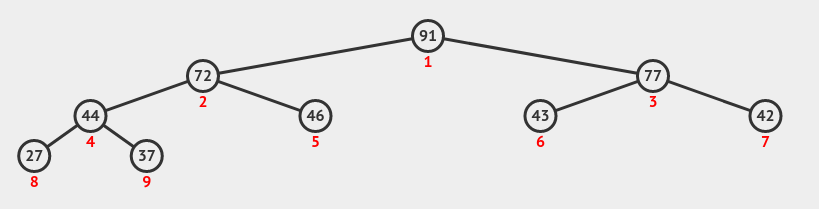
\includegraphics[scale=0.4]{imgs/2.3/heap/heap.png}
    \end{figure}
\end{frame}

\begin{frame}[fragile]{Heap}
    \begin{itemize}
        \item Heap is a \textbf{complete} binary tree: every node, except possibly in the last level, must have both left and right children
    \end{itemize}
	\begin{figure}
        \centering
        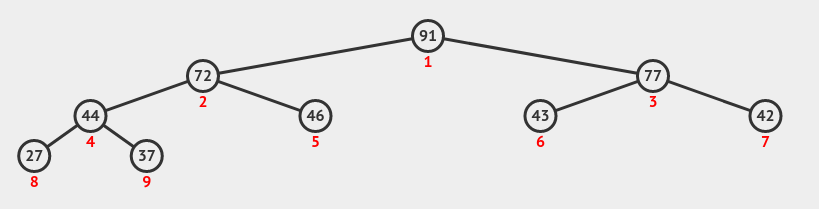
\includegraphics[scale=0.2]{imgs/2.3/heap/heap.png}
    \end{figure}
    
	\begin{itemize}
        \item \textbf{Heap property}: in each subtree rooted at $x$, items on the left and right subtrees of $x$ are smaller (or equal) than $x$
            \begin{itemize}
                \vspace{0.3cm}
                \item This property guarantees that the top element of the Heap (or the root) is the maximum element
                \item There is no notion of \textit{search} in the Heap
                \item Allow for fast deletion of the maximum element and insertion of new items: $O(\log n)$
            \end{itemize}
		\item The height of a Binary Heap of $n$ elements will have a height no taller than $O(\log n)$
    \end{itemize}
\end{frame}

\begin{frame}[fragile]
\frametitle{Heap - Priority Queue ADT}
	\begin{itemize}
		\item The (Max) Heap is useful for modeling a Priority Queue ADT where the item with the highest priority can be dequeued and a new item $v$ can be enqueued in $O(\log n)$
		\item \verb|C++ STL priority_queue|
		\item \color{red} \verb|ch2_06_priority_queue.cpp| \color{black}
	\end{itemize}
\end{frame}

\begin{frame}{Heap - 1D representation}
    \begin{itemize}
        \item Complete binary search trees (Heaps) can be stored in a compact $1$-indexed array of size $n+1$
    \end{itemize}
    
    \vspace{0.2cm}
    \begin{figure}
        \centering
        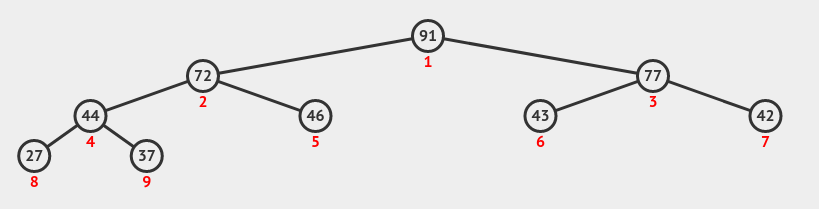
\includegraphics[scale=0.3]{imgs/2.3/heap/heap.png}
        \caption{Heap - Tree Representation}
    \end{figure}
    
    \vspace{0.2cm}
    $$A = [N/A, 91, 72, 77, 44, 46, 43, 42, 27, 37]$$
\end{frame}

\begin{frame}{Heap - 1D representation}
    $$A = [N/A, 91, 72, 77, 44, 46, 43, 42, 27, 37]$$
    \begin{itemize}
        \item Index $0$ is ignored
        \item Operations from index $i$ [\color{blue}bit manipulation\color{black}]:
            \begin{itemize}
                \item Parent: $\left\lfloor \frac{i}{2} \right\rfloor$ or \color{blue}$i \gg 1$ \color{black}
                \item Left child: $2i$ or \color{blue}$i \ll 1$ \color{black}
                \item Right child: $2i+1$, \color{blue}$(i \ll 1)+1$ \color{black}
            \end{itemize}
    \end{itemize}
\end{frame}

\begin{frame}[fragile]
\frametitle{Heap - Operations}
	\begin{itemize}
		\item \verb|insert(v)| - \color{blue} $O(\log n)$ \color{black}
		\item \verb|extract_max()| - \color{blue} $O(\log n)$ \color{black}
		\item \verb|create_heap(A)|
			\begin{itemize}
				\item \color{blue} $O(n)$ \color{black} version
				\item \color{blue} $O(n\log n)$ \color{black} version
			\end{itemize}
		\item \verb|heapsort()| - \color{blue} $O(n\log n)$ \color{black}
	\end{itemize}
\end{frame}

\begin{frame}[fragile]
\frametitle{Heap - Operations: insert(v)}
	\begin{itemize}
		\item Insert new element \verb|v| at the index \verb|n+1|
		\item Move forward in the heap to maintain the heap property
			\begin{itemize}
				\item If the heap property is violated, swap \verb|v| with its parent: \textit{upward fix}
			\end{itemize}
	\end{itemize}
	\begin{lstlisting}[language=c++]
A[A.length] = v;
i = A.length - 1;
while(i > 1 && (A[parent(i)] < i)) {
	swap(A[parent(i)], i);
	i--;
}
\end{lstlisting}
\end{frame}

\begin{frame}[fragile]
\frametitle{Heap - Operations: extract\_max()}
	\begin{itemize}
		\item Read the root of the heap (\verb|A[1]|)
		\item Replace the root with element at \verb|A[n]|
		\item Swap until heap property is satisfied: \textit{downward fix}
	\end{itemize}
	
	\begin{lstlisting}[language=c++]
max_element = A[1]; //read root
A[1] = A[A.length - 1]; //replace with last elememt
i = 1;
A.length--;
// Swap until heap property is satisfied again
while (i < A.length){
	L = max(A[i]->children);
	if (A[i] < L){
		swap(A[i], L);
	}
}
\end{lstlisting}
	\begin{itemize}
		\item Worth noting that \verb|L| is the largest element and not just the left or right children
	\end{itemize}
\end{frame}

\begin{frame}[fragile]
\frametitle{Heap - Operations: create(A)}
	\begin{itemize}
		\item Linear version - \color{blue} $O(n)$ \color{black}
			\begin{itemize}
				\item Starts with an array \verb|A| and assumes it is a binary max heap and then fixes the binary heap property starting from the last internal vertex (\verb|A[A.length/2]|) back to the root
			\end{itemize}
		\item Logarithm version - \color{blue} $O(n\log n)$ \color{black}
			\begin{itemize}
				\item Starts with an empty binary heap and iterates over array \verb|A| by using the \verb|insert(v)| operation
			\end{itemize}
	\end{itemize}
\end{frame}

\begin{frame}[fragile]
\frametitle{Heap - Operations: heapsort()}
	\begin{itemize}
		\item Call \verb|extract_max()| operation \verb|n| times
	\end{itemize}
	
	\vspace{0.6cm}
	
	\begin{lstlisting}[language=c++]
for(i=0; i < A.length; i++)
	extract_max();
\end{lstlisting}	
\end{frame}



%-------------------------------------------------------------------------------------------
%----------------------------------------Hash Table-----------------------------------------
%-------------------------------------------------------------------------------------------
\subsection{Hash Table}
\begin{frame}{Hash Table}
    \begin{figure}
        \centering
        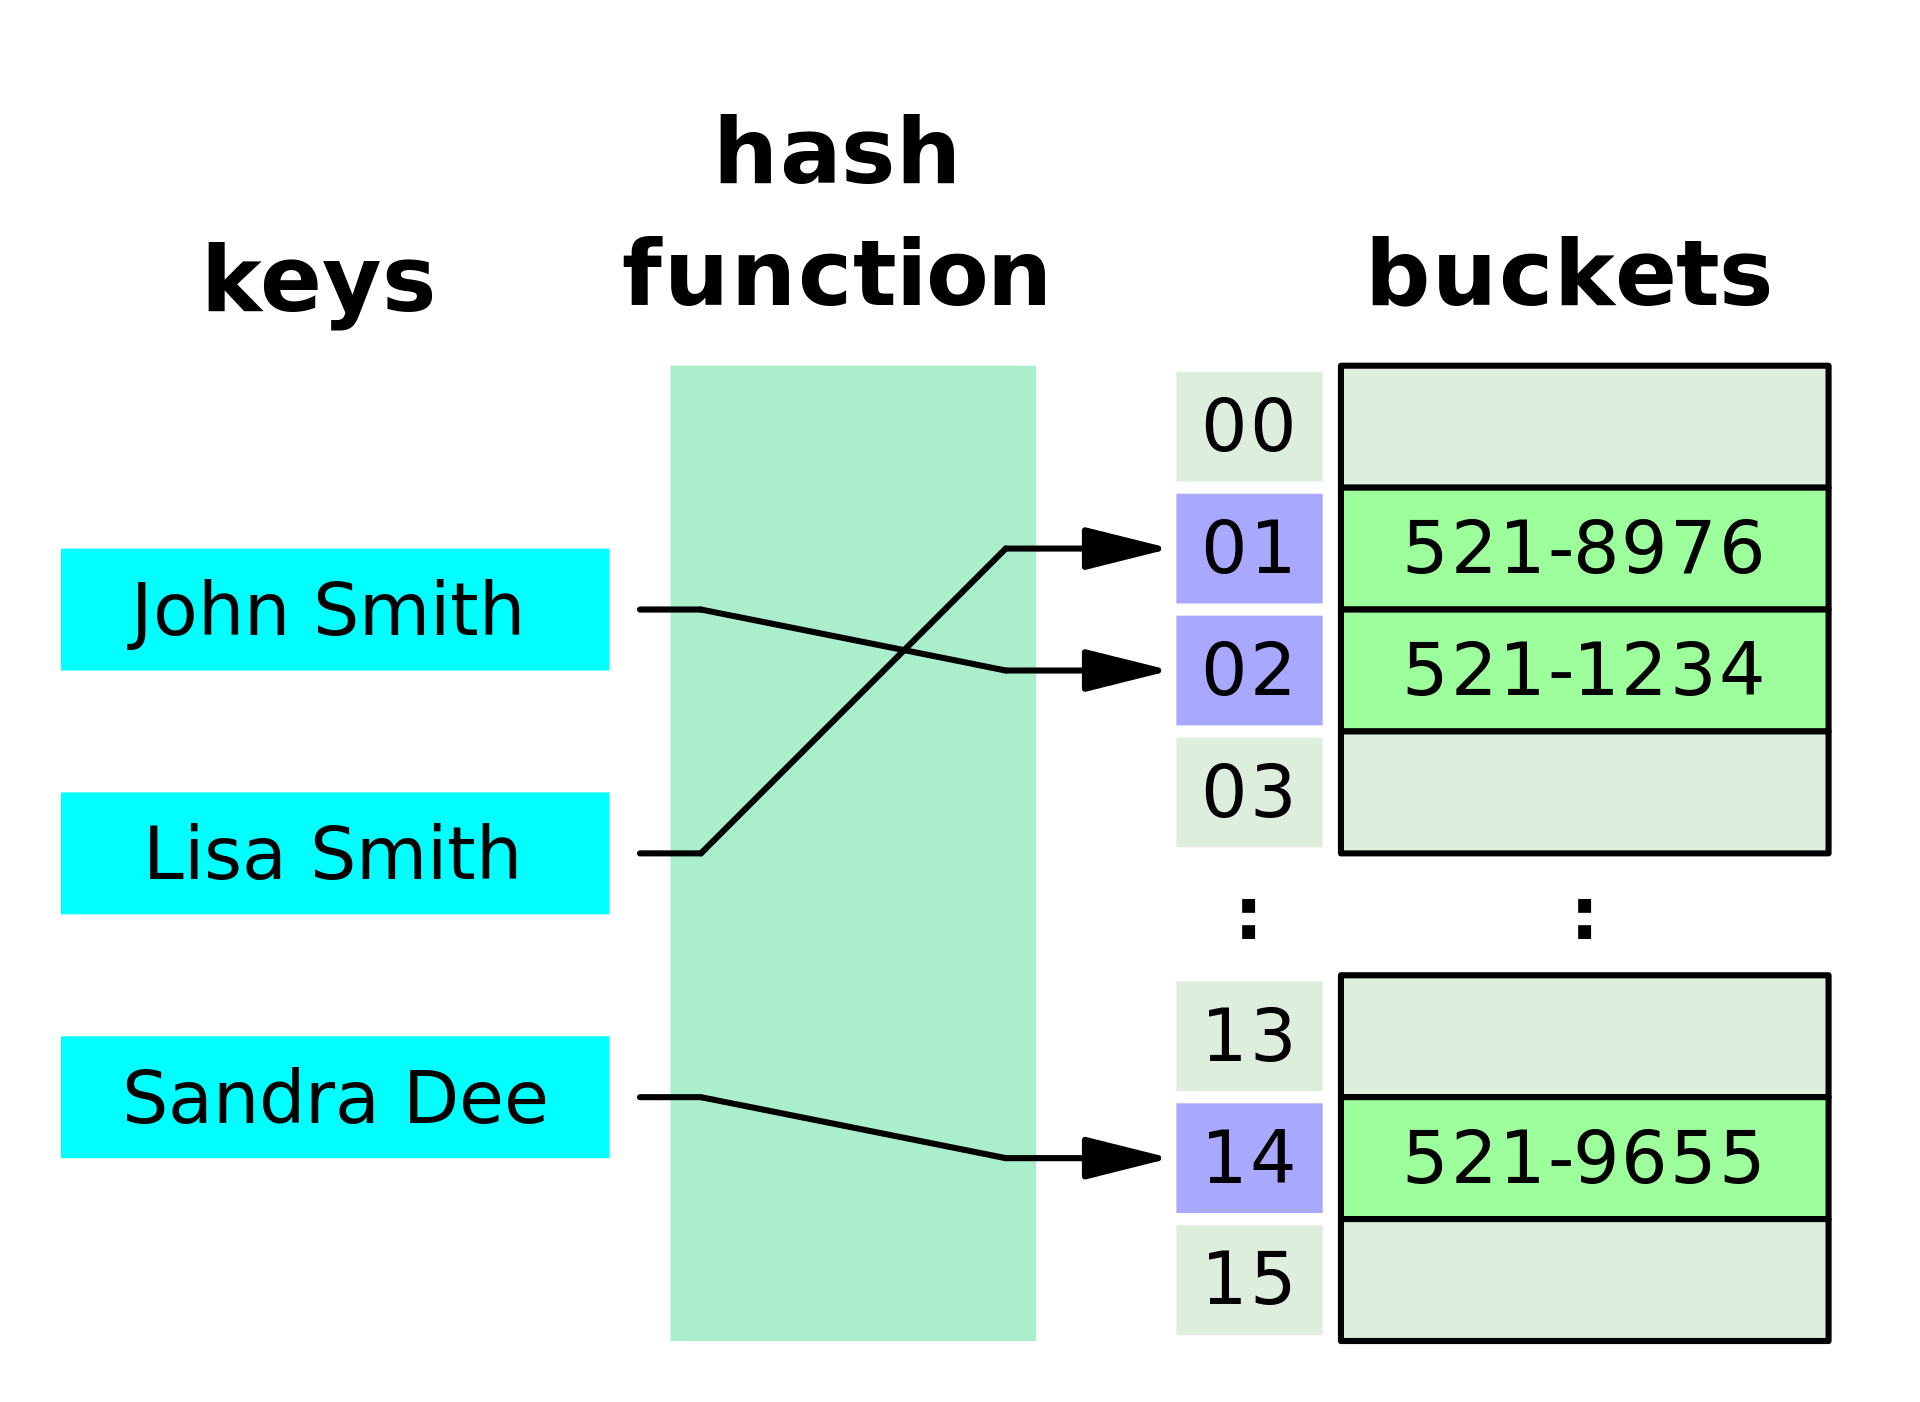
\includegraphics[scale=0.1]{imgs/2.3/hash-table/hash_table.png}
    \end{figure}
\end{frame}

\begin{frame}[fragile]
\frametitle{Hash Table}
	\begin{itemize}
		\item Data structure designed to map key to values
		\item Uses a hash function to map keys into a range of integer indices
	\end{itemize}
	\begin{figure}
		\centering
		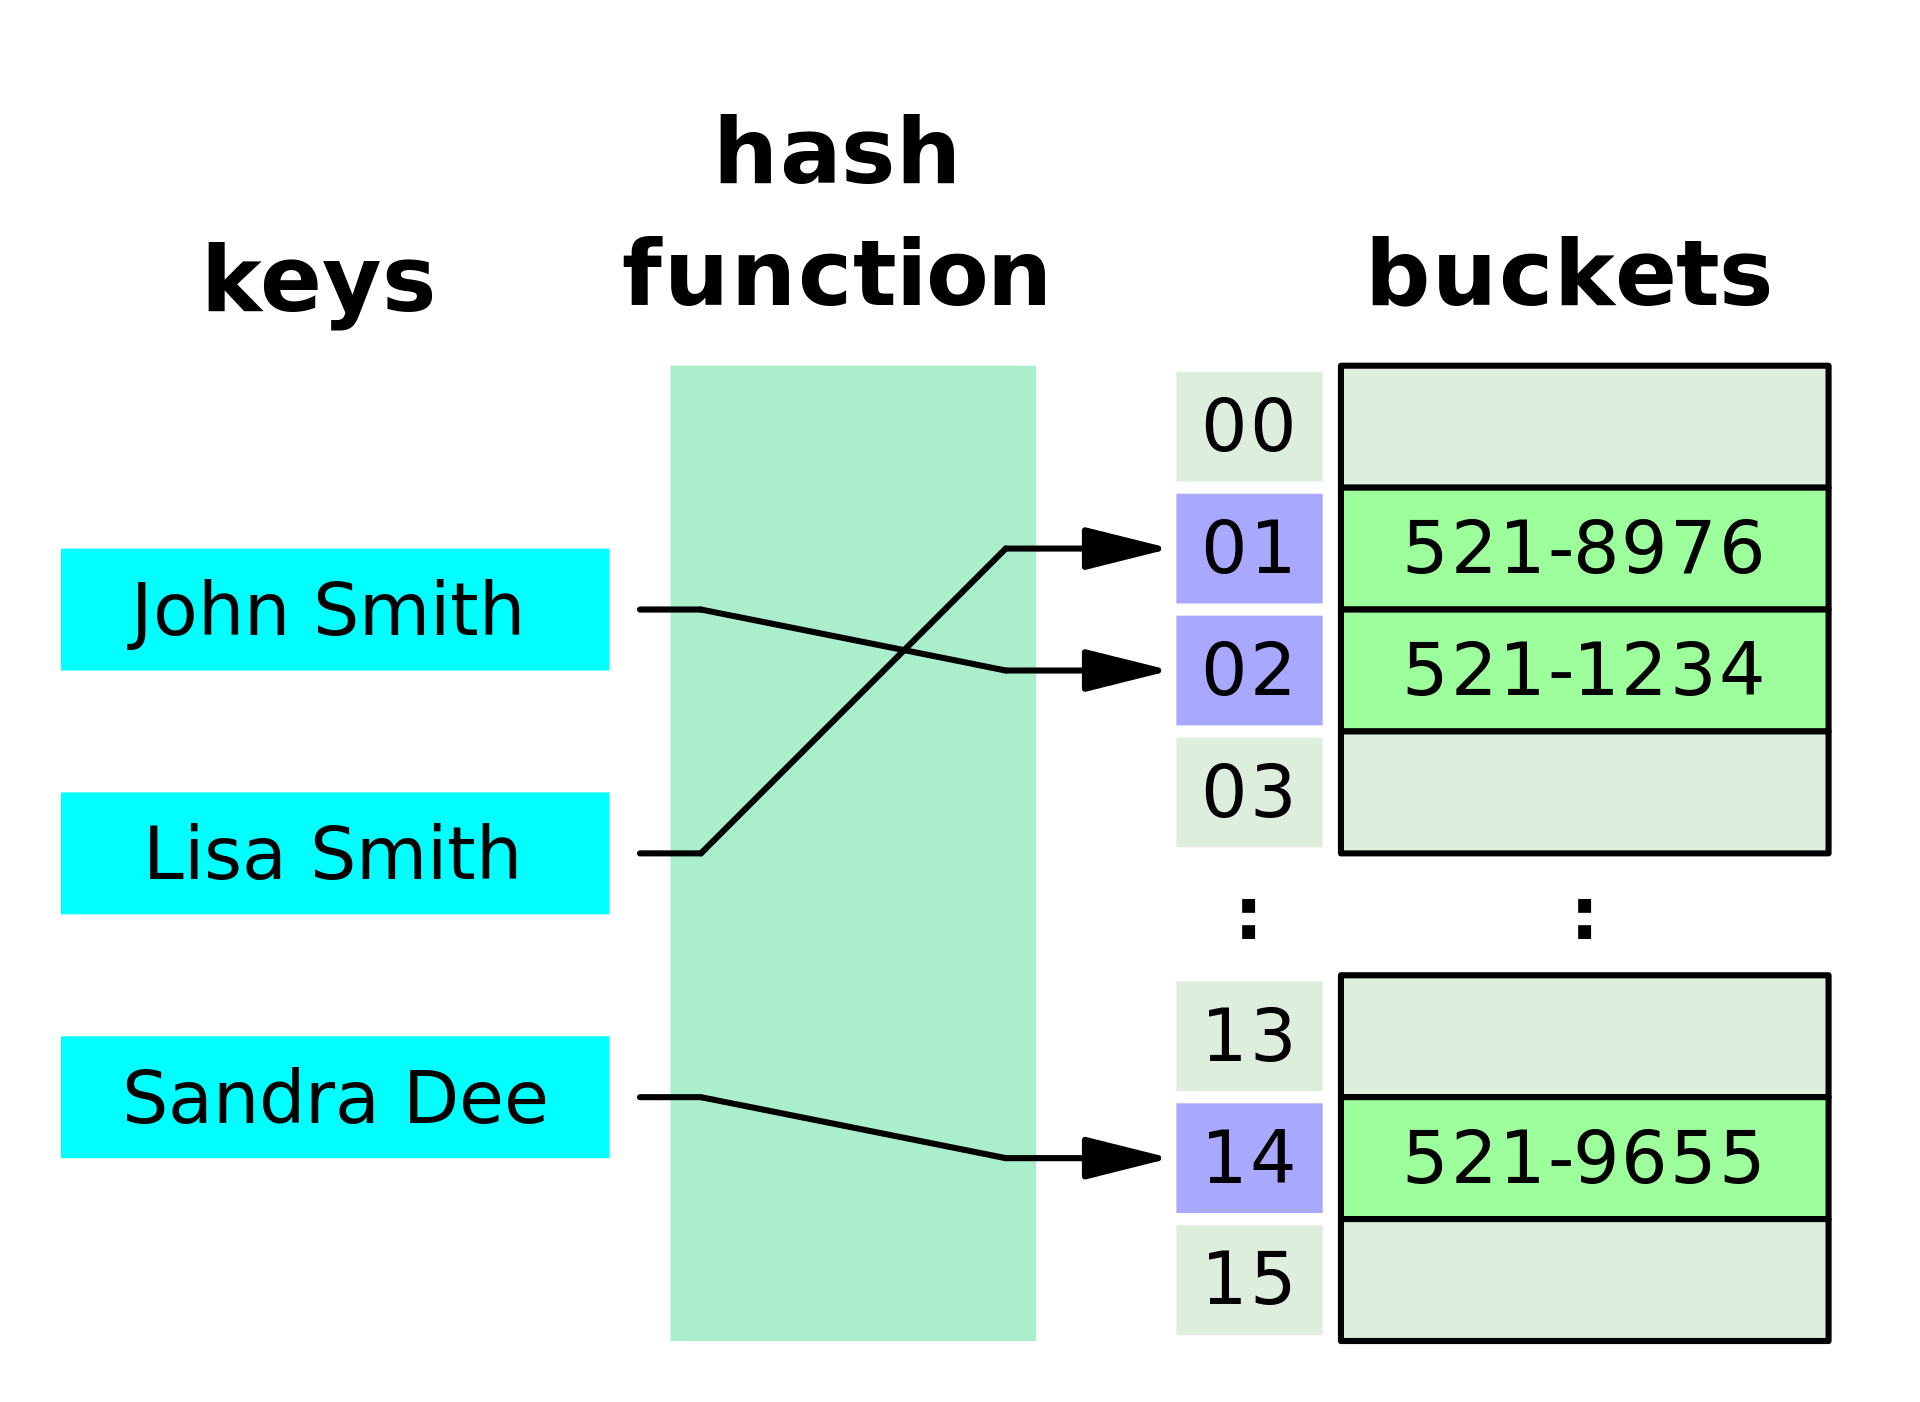
\includegraphics[scale=0.05]{imgs/2.3/hash-table/hash_table.png}
	\end{figure}
	\begin{itemize}
		\item High probability of two items colliding into the same index
		\item Collision resolution strategies:
			\begin{itemize}
				\item Linear Probing
				\item Quadratic Probing
				\item Double Hashing
			\end{itemize}
	\end{itemize}
\end{frame}

\begin{frame}[fragile]
\frametitle{Hash Table - Operations}
	\begin{itemize}
		\item \verb|search(v)|
		\item \verb|insert(v)|
		\item \verb|remove(v)|
	\end{itemize}
	\vspace{0.5cm}
	Implementation via \color{blue}Direct Addressing Table (DAT)\color{black}:
	\begin{itemize}
		\item Initialize and empty boolean array \verb|A| of size \verb|m|:
			\begin{itemize}
				\item \verb|search(v)|: check if \verb|A[v]| is \verb|true| or \verb|false|
				\item \verb|insert(v)|: set \verb|A[v] = true|
				\item \verb|remove(v)|: set \verb|A[v] = false|
			\end{itemize}
		\item Keys cannot be negative and if possible, the range must be small
	\end{itemize}
\end{frame}

\begin{frame}[fragile]
\frametitle{Hash Table - Operations}
	\begin{itemize}
		\item \verb|search(v)|
		\item \verb|insert(v)|
		\item \verb|remove(v)|
	\end{itemize}
	\vspace{0.5cm}
	Implementation via \color{blue}Integer array\color{black}:
	\begin{itemize}
		\item \verb|h(v)| is the hash function applied to the key \verb|v|:
			\begin{itemize}
				\item \verb|search(v)|: check if \verb|A[h(v)] != -1|
				\item \verb|insert(v)|: set \verb|A[h(v)] = v|
				\item \verb|remove(v)|: set \verb|A[h(v)] = -1|
			\end{itemize}
	\end{itemize}
\end{frame}

\begin{frame}[fragile]{Hash Table}
    \begin{itemize}
        \item Not recommended in programming contests unless absolute necessary 
        \item Designing a well performing hash function is hard
        \item \verb|C++ STL map| or \verb|C++ STL set| are usually fast for typical programming contest input ($1M$)
        \item However, Hash Tables are faster: $O(1)$ operations
        \item \verb|C++ STL unordered_map|
    \end{itemize}
\end{frame}


%-------------------------------------------------------------------------------------------
%-------------------------------------------------------------------------------------------
%-------------------------------------------------------------------------------------------
\section{UVa - 2.3}
\begin{frame}{UVa - Competitive Programming 3}
    \begin{itemize}
        \item \textbf{CP3} $>$ \textbf{Data Structures and Libraries} $>$ \textbf{Non Linear Data Structures with Built-in Libraries}
        \item \url{https://onlinejudge.org/index.php?option=com_onlinejudge&Itemid=8&category=630}
    \end{itemize}
\end{frame}


%-------------------------------------------------------------------------------------------
%-------------------------------------------------------------------------------------------
%-------------------------------------------------------------------------------------------
\section{2.4 Data Structures without Libraries}

%-------------------------------------------------------------------------------------------
%-------------------------------------------Graph-------------------------------------------
%-------------------------------------------------------------------------------------------
\subsection{Graph}
\begin{frame}[fragile]
\frametitle{Graph}
	\begin{figure}
		\centering
		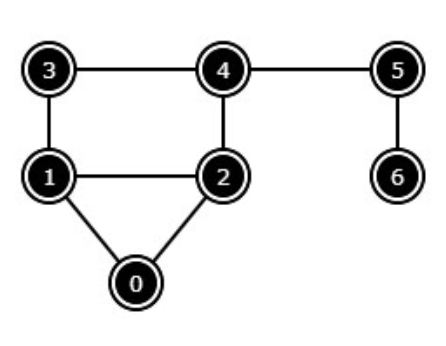
\includegraphics[scale=0.5]{imgs/2.4/graph/graph.png}
	\end{figure}	
\end{frame}

\begin{frame}[fragile]
\frametitle{Graph}
	\begin{itemize}
		\item Set of vertices $(V)$ and edges $(E)$: $G = (V, E)$
	\end{itemize}
	\begin{figure}
		\centering
		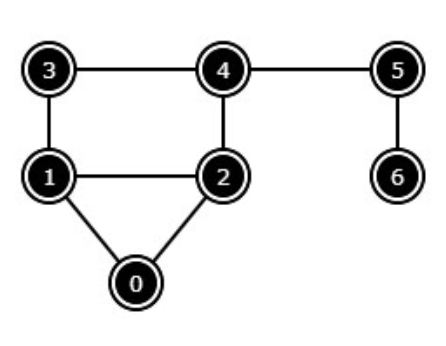
\includegraphics[scale=0.3]{imgs/2.4/graph/graph.png}
	\end{figure}
	\begin{itemize}
		\item Undirected graph: vertices have no direction
		\item Directed graph: vertices have direction
		\item Weighted graph: edges have a numerical values
		\item Unweighted graph: edges do not have numerical values
		\item Simple graph: no loops and no multiple edges between two vertices	
		\item \color{red}\verb|ch_07_graph.cpp|\color{black}
	\end{itemize}
\end{frame}

\begin{frame}[fragile]
\frametitle{Graph - Terminology I}
	\begin{itemize}
		\item An undirected edge $e:(u,v)$ is said to be \textbf{incident} with its two end-point vertices: $u$ and $v$
		\item Two vertices are called \textbf{neighbors} if they are incident with a common edge
	\end{itemize}
	\begin{figure}
		\centering
		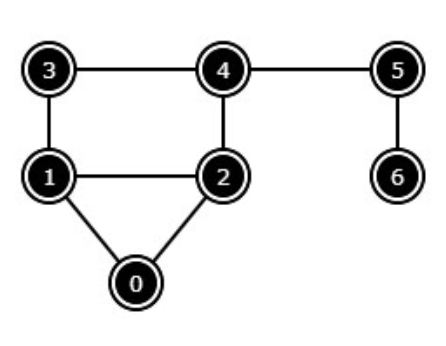
\includegraphics[scale=0.4]{imgs/2.4/graph/graph.png}
	\end{figure}
	\begin{itemize}
		\item Vertices $0$ and $2$ are neighbors
		\item The \textbf{degree} of vertex $v$ in an undirected graph is the number of edges incident with $v$
	\end{itemize}
\end{frame}

\begin{frame}[fragile]
\frametitle{Graph - Terminology II}
	\begin{itemize}
		\item A \textbf{path} in an undirected graph $G$ is a sequence of vertices such that there is an edge between $v_i$ and $v_{i+1} \; \forall i \in [0,\ldots,n-1]$
	\end{itemize}
	\begin{figure}
		\centering
		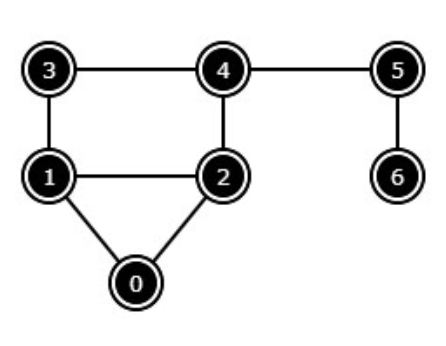
\includegraphics[scale=0.4]{imgs/2.4/graph/graph.png}
	\end{figure}
	\begin{itemize}
		\item One possible path: $0,1,3,4,5$
		\item A \textbf{simple path} is a path where vertices are not repeated
	\end{itemize}
\end{frame}

\begin{frame}[fragile]
\frametitle{Graph - Terminology III}
	\begin{itemize}
		\item An undirected graph $G$ is called \textbf{connected} if there is a path between every pair of distinct vertices of $G$
	\end{itemize}
	\begin{figure}
		\centering
		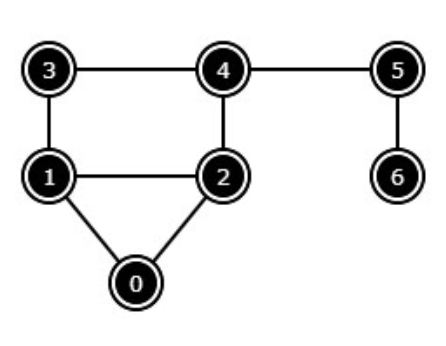
\includegraphics[scale=0.4]{imgs/2.4/graph/graph.png}
		\caption{Connected graph}
	\end{figure}
\end{frame}

\begin{frame}
\frametitle{Graph - Terminology IV}
\begin{itemize}
\item
An undirected graph $C$ is a \textbf{connected component} of the undirected graph $G$ if:
	\begin{enumerate}
	\item
	$C$ is a subgraph of $G$
	\item
	$C$ is connected
	\item
	No connected subgraph of $G$ has $C$ as a subgraph and contains vertices or edges that are not in $C$
	\end{enumerate}
\end{itemize}
	\vspace{0.4cm}
	
	\begin{figure}
	\centering
	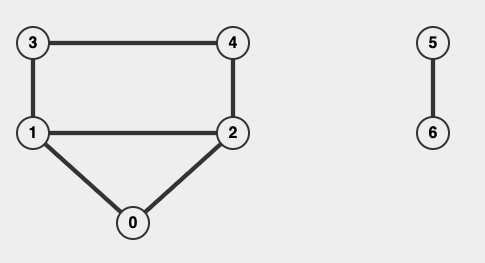
\includegraphics[scale=0.25]{imgs/2.4/graph/connected-components.png}
	\caption{Graph $G$ with two connected components}
	
	\end{figure}
\end{frame}

\begin{frame}
\frametitle{Graph - Terminology V}
Adjustments for directed graphs:
\begin{itemize}
	\item If we have a directed edge $e: (u\rightarrow v)$ we say that $v$ is adjacent to $u$ but not necessarily the other way around
	\item We have to differentiate the \textbf{degree} of a vertex into \textit{in-degree} and \textit{out-degree}
\end{itemize}

\begin{figure}
    \centering
    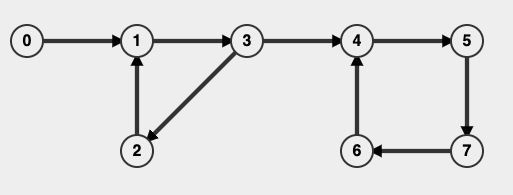
\includegraphics[scale=0.3]{imgs/2.4/graph/directed-graph.png}
\end{figure}

\end{frame}

\begin{frame}[fragile]
\frametitle{Graph - Terminology VI}

\begin{itemize}
\item A directed graph is \textbf{strongly connected} if there is a path in each direction between each pair of vertices, i.e., every vertex is reachable from every other vertex
\item A \textbf{strongly connected component} is a subgraph of a directed graph that is strongly connected
\end{itemize}

\begin{figure}
	\centering
	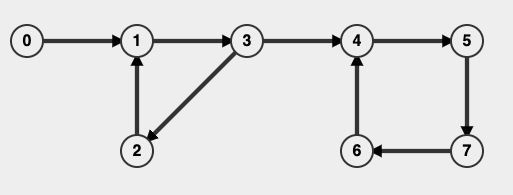
\includegraphics[scale=0.3]{imgs/2.4/graph/directed-graph.png}
\end{figure}
\end{frame}

\begin{frame}
\frametitle{Graph - Terminology VII}
	\begin{itemize}
	    \item \textbf{Cycle}: path that starts and ends in the same vertex
	    \item \textbf{Acyclic graph}: graph that does not contains cycles
	    \item \textbf{Directed Acyclic Graph (DAG)}: directed graph that is also acyclic
	\end{itemize}
\end{frame}

\begin{frame}
\frametitle{Graph - Termninology VII}
	Types of graphs:
	\begin{enumerate}
	    \item Undirected - Unweighted
	    \item Undirected - Weighted
	    \item Directed - Unweighted
	    \item Directed - Weighted
	\end{enumerate}
\end{frame}

\begin{frame}
\frametitle{Example 1: social network}
	\begin{itemize}
	    \item Vertices can represent people and edges the connection between them
	    \item Who is friend with who? Who has the most friends? Is there any isolated people? Is there a common friend between two strangers?
	\end{itemize}
	\begin{figure}
	    \centering
	    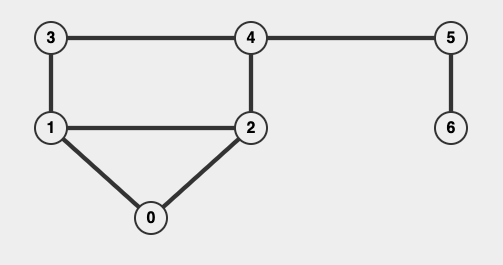
\includegraphics[scale=0.3]{imgs/2.4/graph/social-network.png}
	\end{figure}
\end{frame}

\begin{frame}
\frametitle{Example 2: transportation network}
	\begin{itemize}
	    \item Vertices represents stations and edges connection between them (roads with weights)
	    \item What is the path with the least amount of time between station 0 and station 4?
	\end{itemize}
	
	\begin{figure}
	    \centering
	    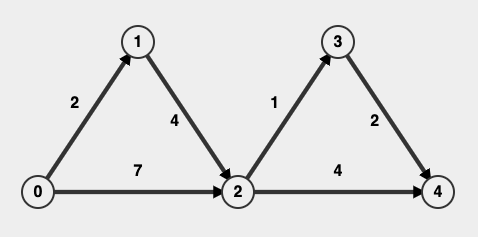
\includegraphics[scale=0.3]{imgs/2.4/graph/transportation-network.png}
	\end{figure}
\end{frame}

\begin{frame}
\frametitle{Special Graphs I: Rooted Tree}
	\begin{itemize}
	    \item \textbf{Connected} and \textbf{acyclic} graph with $V$ vertices and $E = V-1$ edges
	    \item One \textbf{unique} path between any pair of vertices
	\end{itemize}
	\begin{figure}
	    \centering
	    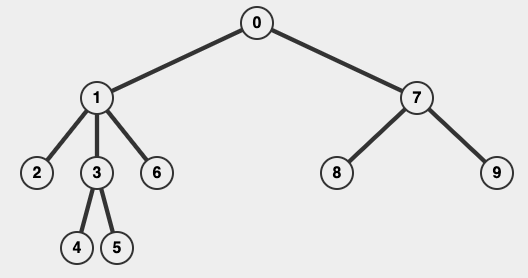
\includegraphics[scale=0.3]{imgs/2.4/graph/tree-one.png}
	    \caption{Rooted tree}
	\end{figure}
\end{frame}

\begin{frame}
\frametitle{Special Graphs I: Non Rooted Tree}
	\begin{itemize}
	    \item Not all trees are drawn with a root vertex at top and leaf vertices at the bottom
	\end{itemize}
	\begin{figure}
	    \centering
	    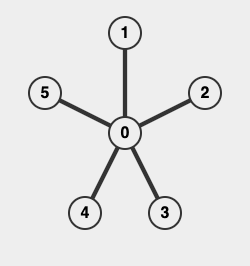
\includegraphics[scale=0.4]{imgs/2.4/graph/tree-two.png}
	    \caption{Non rooted tree}
	\end{figure}
\end{frame}

\begin{frame}[fragile]
\frametitle{Special Graphs I: Binary Tree}
	\begin{itemize}
	    \item Rooted tree in which every vertex hast at most two children (\verb|left| and \verb|right|)
	    \item \textbf{Full binary tree}: binary tree in which every non-leaf node has exactly two children
	    \item \textbf{Complete binary tree}: binary tree in which every level is completely filled
	\end{itemize}
	\begin{figure}
	    \centering
	    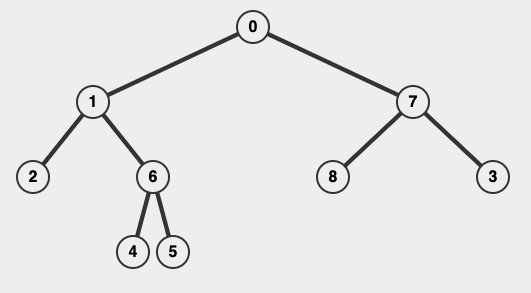
\includegraphics[scale=0.2]{imgs/2.4/graph/full-binary-tree.png}
	    \caption{Full binary tree}
	\end{figure}
\end{frame}

\begin{frame}
\frametitle{Special Graphs II: Complete graph}
	\begin{itemize}
	    \item Graph with $V$ vertices and $E = \frac{V(V-1)}{2}$ edges
	    \item There is an edge between any pair of vertices
	\end{itemize}
	
	\begin{figure}
	    \centering
	    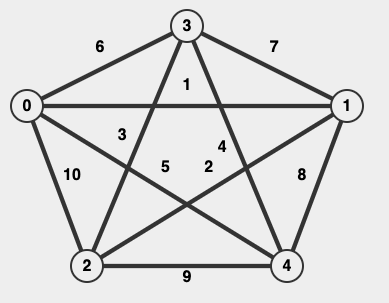
\includegraphics[scale=0.3]{imgs/2.4/graph/complete-graph.png}
	\end{figure}
\end{frame}

\begin{frame}
\frametitle{Special Graphs III: Bipartite}
	\begin{itemize}
	    \item Undirected graph with $V$ vertices that can be partitioned into two disjoint sets of size $m$ and $n$ where $V = m + n$
	    \item There is no edge between members of the same set
	    \item Bipartite graph can also be complete
	\end{itemize}
	\begin{figure}
	    \centering
	    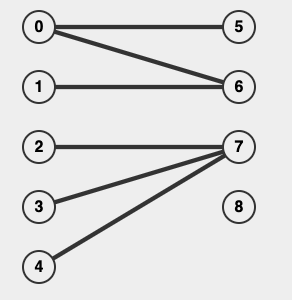
\includegraphics[scale=0.35]{imgs/2.4/graph/bipartite.png}
	\end{figure}
\end{frame}

\begin{frame}
\frametitle{Special Graphs IV: DAG}
	\begin{itemize}
	    \item Directed acyclic graphs
	    \item Each DAG has at least one topological order
	\end{itemize}
	\begin{figure}
	    \centering
	    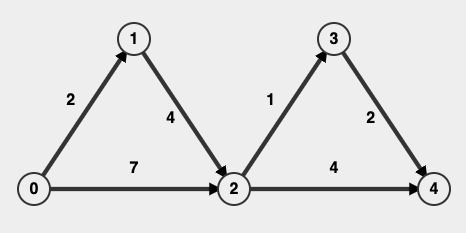
\includegraphics[scale=0.35]{imgs/2.4/graph/dag.png}
	\end{figure}
\end{frame}

\begin{frame}
\frametitle{Graph as a Data Structure}
		There are three main ways to store a graph (nodes, edges) in a data structure, \color{blue} \huge{can you think of one?} \color{black}
\end{frame}

\begin{frame}
\frametitle{Graph as a Data Structure}
	Main ways to store a graph in a data structure:
	\begin{enumerate}
	    \item Adjacency Matrix
	    \item Adjacency List
	    \item Edge List
	\end{enumerate}
\end{frame}

\begin{frame}[fragile]
\frametitle{1. Adjacency Matrix}
	\begin{itemize}
	    \item An adjacency matrix $M$ is a square matrix where the entry $M[i][j]$ corresponds to the edge's weight from vertex $i$ to vertex $j$
	    \item For unweighted graphs we can set a unit weight $1$ for all edges
	\end{itemize}
	\begin{figure}
	    \centering
	    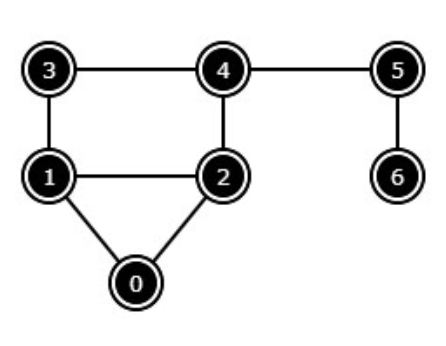
\includegraphics[scale=0.45]{imgs/2.4/graph/graph.png}
	    \hspace{0.4cm}
	    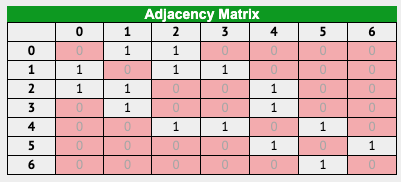
\includegraphics[scale=0.4]{imgs/2.4/graph/adjacency-matrix.png}	    
	\end{figure}
	\begin{itemize}
	    \item We simply use a $2\times2$\verb| C++ array|
	    \item Space: $O(V^2)$ where $V$ is the number of vertices
	\end{itemize}
\end{frame}

\begin{frame}[fragile]
\frametitle{2. Adjacency List}
	\begin{itemize}
	    \item Array $L$ of $V$ lists, on for each vertex
	    \item $L[i]$ stores the list of vertex $i$'s neighbors
	    \item Space: $O(V+E)$. Much more efficient than adjacency matrix $M$
	\end{itemize}
	\begin{figure}
	    \centering
	    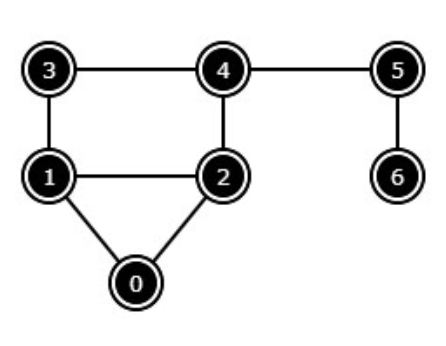
\includegraphics[scale=0.45]{imgs/2.4/graph/graph.png}
	    \hspace{0.4cm}
	    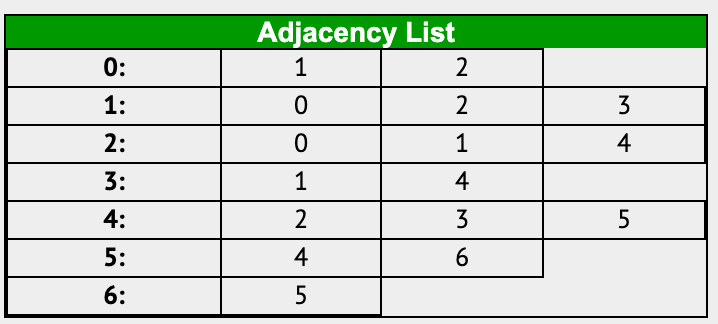
\includegraphics[scale=0.4]{imgs/2.4/graph/adjacency-list.png}	    
	\end{figure}
\end{frame}

\begin{frame}[fragile]
\frametitle{3. Edge List}
	\begin{itemize}
	    \item $E$ is a collection of edges with both connecting vertices and their weights
	    \item Usually the edges are sorted by increasing weight
	\end{itemize}
\end{frame}

%-------------------------------------------------------------------------------------------
%----------------------------------------Union-Find-----------------------------------------
%-------------------------------------------------------------------------------------------
\subsection{Union-Find Disjoint Sets}

\begin{frame}
\frametitle{Union-Find Disjoint Sets (UFDS)}
	\begin{figure}
	    \centering
	    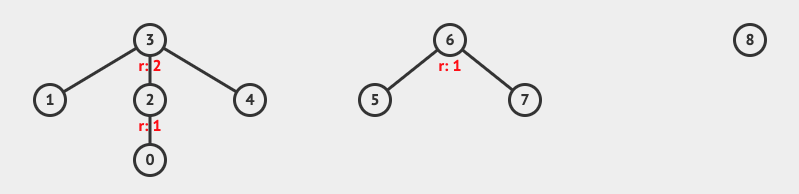
\includegraphics[scale=0.38]{imgs/2.4/ufds/ufds.png}
	\end{figure}
\end{frame}

\begin{frame}[fragile]
\frametitle{Union-Find Disjoint Sets}
	\begin{itemize}
	    \item Data structure to model a collection of disjoint sets \footnote{Two sets are disjoint if they have no element in common} with the ability to efficiently (in $O(1)$):
	    	\begin{enumerate}
			    \item Determine which set an item belongs to
			    \item Unite two disjoint sets into one larger set
			\end{enumerate}
	\end{itemize}
	\begin{figure}
	    \centering
	    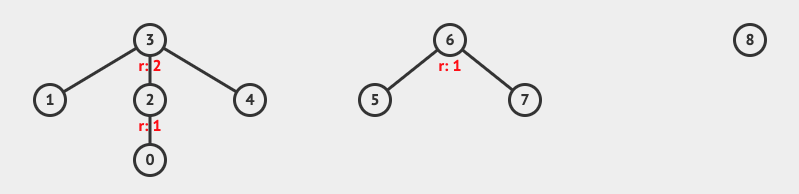
\includegraphics[scale=0.2]{imgs/2.4/ufds/ufds.png}
	\end{figure}
	\begin{itemize}		
		\item Applications: finding connected components in an undirected graph
		\item \color{red}\verb|ch2_08_unionfind_ds.cpp|\color{black}
	\end{itemize}
\end{frame}

\begin{frame}[fragile]
\frametitle{UFDS intuition}
	\begin{itemize}
		\item Disjoint sets are represented as trees
	    \item Each disjoint set has a representative item (root of the tree)
	    \item UFDS creates a tree structure where the disjoint sets form a forest
	\end{itemize}
\end{frame}

\begin{frame}[fragile]
\frametitle{UFDS - Example}
	\begin{itemize}
	    \item 5 disjoint sets: $\{0,1,2,3,4\}$
	\end{itemize}
	\begin{figure}
	    \centering
	    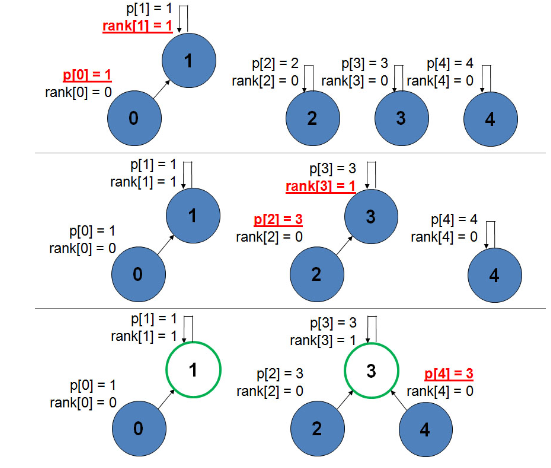
\includegraphics[scale=0.3]{imgs/2.4/ufds/example-1.png}
	\end{figure}
\end{frame}

\begin{frame}[fragile]
\frametitle{UFDS - Example (continuation)}
	\begin{figure}
	    \centering
	    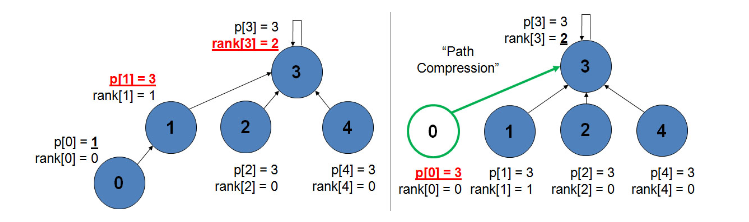
\includegraphics[scale=0.4]{imgs/2.4/ufds/example-2.png}
	\end{figure}
\end{frame}

\begin{frame}[fragile]
\frametitle{UFDS - Operations}
	\begin{itemize}
		\item Each node of the tree contains these two elements:
			\begin{enumerate}
			    \item \color{blue}\verb|p|\color{black}: index of the representative item			
			    \item \color{blue}\verb|rank|\color{black}: height of the disjoint set
			\end{enumerate}
	    \item \color{blue}\verb|unionSet(i,j)|\color{black}: unites to disjoint sets by setting the representative item (root) of one disjoint set to be the new parent of the representative item of the other disjoint set. This will cause that both $i$ and $j$ have the same representative item
	    \item \color{blue}\verb|findSet(i)|\color{black}: finds the representative item for node $i$
	    \item \color{blue}\verb|isSameSet(i,j)|\color{black}: determines if items $i$ and $j$ belong to the same set. This can be done by calling \verb|findSet(i)| and \verb|findSet(j)| and checking if both are equal
	\end{itemize}
\end{frame}


%-------------------------------------------------------------------------------------------
%---------------------------------------Segment Tree----------------------------------------
%-------------------------------------------------------------------------------------------
\subsection{Segment Tree}

\begin{frame}[fragile]
\frametitle{Segment Tree}
	\begin{figure}
	    \centering
	    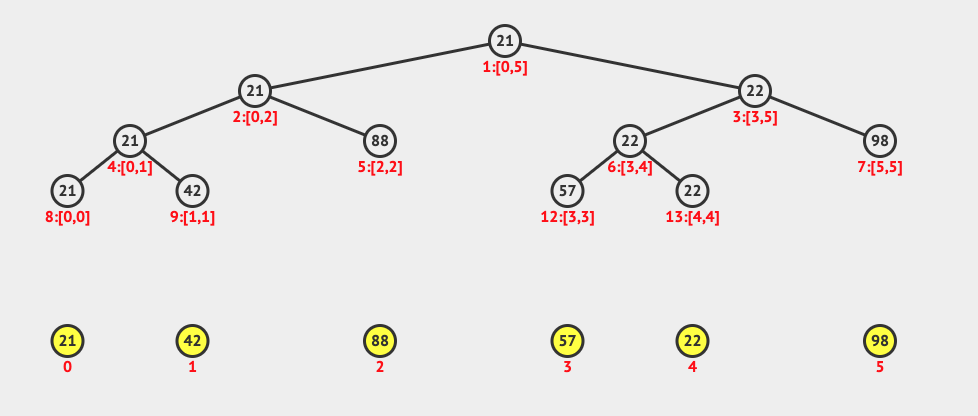
\includegraphics[scale=0.3]{imgs/2.4/segment-tree/segment-tree.png}
	\end{figure}
\end{frame}

\begin{frame}[fragile]
\frametitle{Segment Tree}
	\begin{itemize}
	    \item Data structure that can efficiently answer dynamic \footnote{Dynamic problems are the ones in which we need to frequently update the data; thus, making pre-processing techniques useless} range queries
	\end{itemize}
	\begin{figure}
	    \centering
	    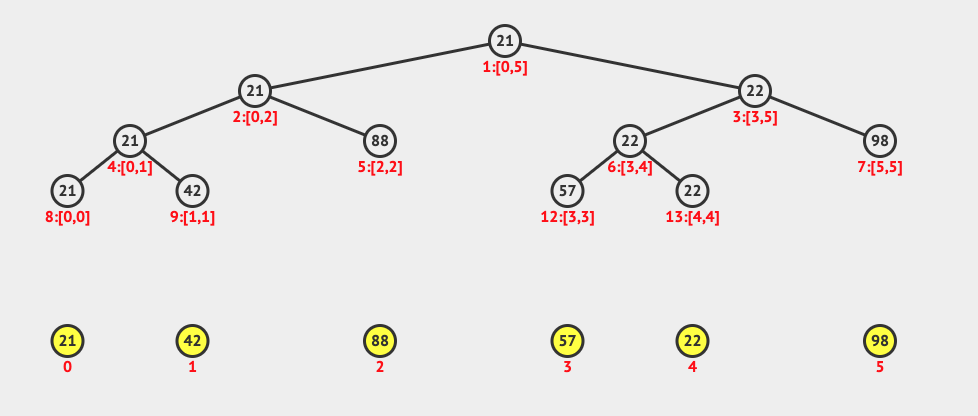
\includegraphics[scale=0.15]{imgs/2.4/segment-tree/segment-tree.png}
	\end{figure}
	\begin{itemize}
	    \item One example of range queries is the problem of finding the index of the minimum element in the array within a range \verb|[i,j]|. This problem is called Range Minimum Query (RMQ)
	    \item \color{red}\verb|ch2_09_segmenttree_ds.cpp|\color{black}
	\end{itemize}
\end{frame}

\begin{frame}[fragile]
\frametitle{Segment Tree - Implementation}
	\begin{itemize}
		\item \verb|build| routine ($O(2n)$):
			\begin{itemize}
	    		\item $1$-based compact array \verb|st| where index 1 is the root and the left and right children of index $p$ are indices $2\cdot p$ and $(2\cdot p)+1$ respectively
			    \item The value of \verb|st[p]| is the RMQ value of the segment associated with index \verb|p|
	    		\item The root (index 1 of \verb|st|) represents segment \verb|[0,n-1]|
			    \item For each segment \verb|[L,R]| stored in index \verb|p| where \verb|L!=R|, the segment will be split into \verb|[L, (L+R)/2]| and \verb|[(L+R)/2+1, R]|
			\end{itemize}
	\end{itemize}
\end{frame}

\begin{frame}[fragile]
\frametitle{Segment Tree - Implementation II}
	\begin{itemize}
	    \item Answering an RMQ can be done in $O(\log n)$
	    \item \verb|RMQ(i,i) = i| where \verb|i| is an index of \verb|st|
	    \item \verb|RMQ(i,j)| where \verb|i!=j|:
	    	\begin{itemize}
			    \item \verb|rmq| routine:
			    	\begin{itemize}
					    \item Let \verb|p1=rmq(i, (i+j)/2)| and \verb|p2=rmq((i+j)/2+1,j)|
					    \item \verb|RMQ(i,j)| will be \verb|p1| if \verb|st[p1] <= st[p2]| or \verb|p2| otherwise
					\end{itemize}
			\end{itemize}
	\end{itemize}
\end{frame}


%-------------------------------------------------------------------------------------------
%---------------------------------------Fenwick-Tree----------------------------------------
%-------------------------------------------------------------------------------------------
\subsection{Binary Indexed (Fenwick) Tree}

\begin{frame}[fragile]
\frametitle{Binary Indexed (Fenwick) Tree}
	\begin{figure}
	    \centering
	    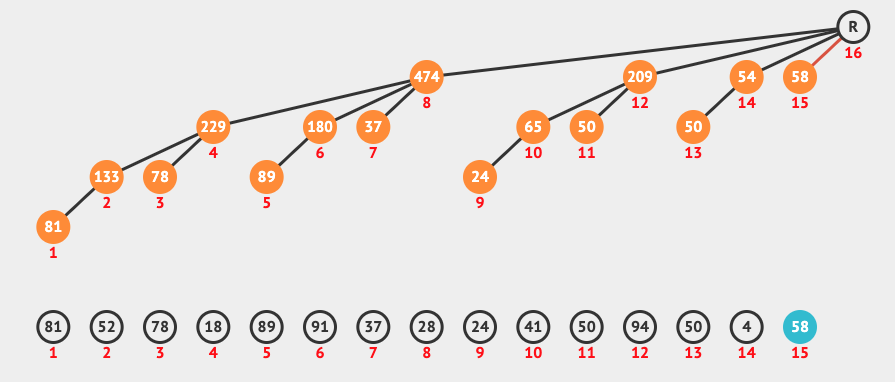
\includegraphics[scale=0.3]{imgs/2.4/fenwick-tree/fenwick-tree.png}
	\end{figure}
\end{frame}

\begin{frame}[fragile]
\frametitle{Binary Indexed (Fenwick) Tree}
	\begin{itemize}
	    \item Invented by Peter Fenwick in 1984
	    \item Useful data structure for implementing dynamic cumulative frequency tables (see example on the next slide)
	    \item Fenwick tree operations are extremely efficient since the use bit manipulation techniques
	\end{itemize}
	\begin{figure}
	    \centering
	    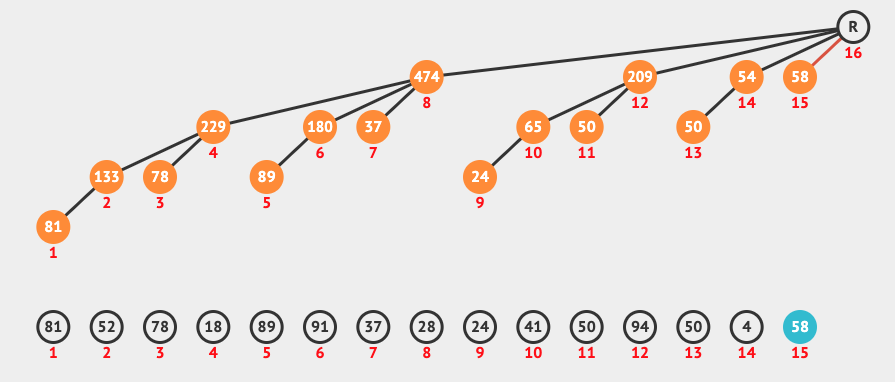
\includegraphics[scale=0.2]{imgs/2.4/fenwick-tree/fenwick-tree.png}
	\end{figure}
	\begin{itemize}
	    \item \color{red}\verb|ch2_10_fenwicktree_ds.cpp|\color{black}
	\end{itemize}
\end{frame}

\begin{frame}[fragile]
\frametitle{Fenwick Tree - Example}
	\begin{itemize}
	    \item Suppose we have the test scores of \verb|m=11| students
	    \item \verb|f={2,4,5,5,6,6,6,7,7,8,9}|
	    \item Test scores are integer values in \verb|[1,10]|
	\end{itemize}
	\begin{figure}
	    \centering
	    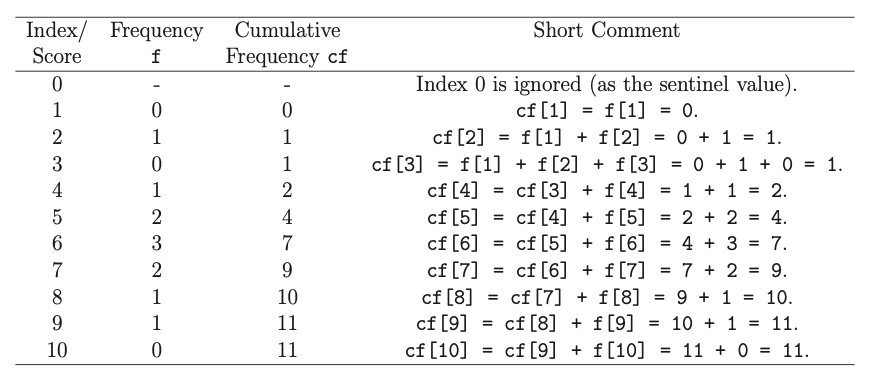
\includegraphics[scale=0.25]{imgs/2.4/fenwick-tree/ft.png}
	\end{figure}
	\begin{itemize}
	    \item The problem becomes evident if the frequency of previously seen scores suffers an update. In this case, we would have to start all over again from the start in $O(n)$ time
	\end{itemize}
\end{frame}

\begin{frame}[fragile]
\frametitle{Fenwick Tree - Implementation}
	\begin{itemize}
	    \item Typically implemented as a dynamic array (vector)
	    \item A Fenwick Tree \verb|ft| is a tree indexed bi the bits of its integer keys
	    	\begin{itemize}
			    \item The keys fall within a fixed range \verb|[1,n]| \footnote{Note that we skip index 0}
			\end{itemize}
		\item The element at index \verb|i| is responsible for elements in the range \verb|[i-LSOne(i)+1..i]|
		\item \verb|ft[i]| stores the cumulative frequency of elements \verb|{i-LSOne(i)+1, i-LSOne(i)+2, i-LSOne(i)+3, ..., i}|
		\item \verb|LSOne(i) = (i & (-i))| produces the Least Significant One-bit in \verb|i|
	\end{itemize}
\end{frame}

\begin{frame}[fragile]
\frametitle{Fenwick Tree - Implementation II}
	\begin{itemize}
	    \item If we want to obtain the cumulative frequency between \verb|[1,...,b]|, we simply add \verb|ft[b],ft[b'],ft[b''],...| until index $b^i$ is $0$
	    \item \verb|b' = b - LSOne(b)|
	    \item This process runs in $O(\log n)$ when \verb|b=n|
	\end{itemize}
	\begin{figure}
	    \centering
	    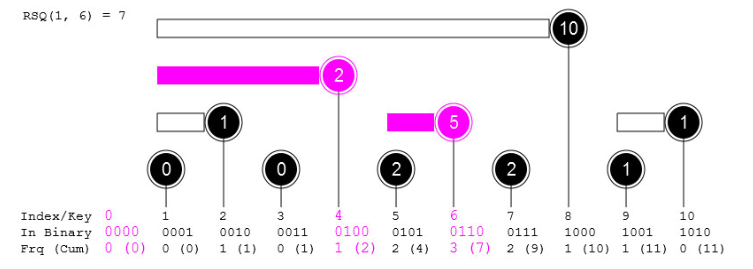
\includegraphics[scale=0.3]{imgs/2.4/fenwick-tree/rsq.png}
	\end{figure}
	\begin{itemize}
	    \item To evaluate the cumulative frequency between two indices \verb|[a...b]| where \verb|a != 1| we simply evaluate \verb|rsq(a, b) = rsq(b) - rsq(a-1)|
	\end{itemize}
\end{frame}

%-------------------------------------------------------------------------------------------
%-------------------------------------------------------------------------------------------
%-------------------------------------------------------------------------------------------
\section{UVa - 2.4}
\begin{frame}{UVa - Competitive Programming 3}
    \begin{itemize}
        \item \textbf{CP3} $>$ \textbf{Data Structures and Libraries} $>$ \textbf{Data Structures with Our-Own Libraries}
        \item \url{https://onlinejudge.org/index.php?option=com_onlinejudge&Itemid=8&category=634}
    \end{itemize}
\end{frame}


%-------------------------------------------------------------------------------------------
%-------------------------------------------------------------------------------------------
%-------------------------------------------------------------------------------------------
%\section{Extra: DFS and BFS}
%\begin{frame}{DFS}
    
%\end{frame}

%\begin{frame}{BFS}
    
%\end{frame}


%-------------------------------------------------------------------------------------------
%-------------------------------------------------------------------------------------------
%-------------------------------------------------------------------------------------------
\section*{References}
\begin{frame}{References}
    \begin{thebibliography}{}
        \bibitem[Halim]{Halim} Halim S., Halim F., \textit{Competitive Programming 3}, Handbook for ACM ICPC and IOI Contestants. 2013
        \bibitem[Stroustrup]{Stroustrup} Stroustrup B. \textit{The C++ Programming Language}. Fourth ed. 
        \bibitem{skiena} Skiena S. \textit{The Algorithm Design Manual}. Springer. 2020
    \end{thebibliography}
\end{frame}

\end{document}
